\documentclass[11pt,a4paper]{article}
\usepackage[hyperref]{acl2018}
\usepackage{times}
\usepackage{latexsym}
\usepackage{graphicx}
\usepackage{url}

\aclfinalcopy % Uncomment this line for the final submission
%\def\aclpaperid{***} %  Enter the acl Paper ID here

%\setlength\titlebox{5cm}
% You can expand the titlebox if you need extra space
% to show all the authors. Please do not make the titlebox
% smaller than 5cm (the original size); we will check this
% in the camera-ready version and ask you to change it back.

\newcommand\BibTeX{B{\sc ib}\TeX}

\title{Optimization Method Coding Project 2: \\ Conjugate Gradient Methods}

\author{Li, Ziyao \\
  1500017776 / Yuanpei College \\
  {\tt leeeezy@pku.edu.cn}
  }

\date{}

\begin{document}
\maketitle
\begin{abstract}
  This work focuses on the realization of Conjugate Gradient and Global BB Methods. Three test functions are evaluated in this work, namely Generalized BARD Function, Generalized CUBE Function and s303-305 Function. Numerical Experiments are conducted on three formerly mentioned problems. Generally FR and PRP methods takes less iterations than other CG and GBB (Global BB) methods, while adopting a non-monotone line search method, GBB do significantly out-perform CGs with regard to Generalized CUBE Function.
\end{abstract}

\section{Conjugate Gradient Methods}

Generally the Conjugate Gradient Methods introduce the direction of last iteration when calculating a descend direction, i.e.
\begin{displaymath}
  d_k = -g_k + \beta_{k-1} d_{k-1}.
\end{displaymath}
The differences of the variety of CG Methods diverge over the calculation of the proportion, i.e. $\beta$ in the above formula. Five different CG methods are examined in this report with formulas:
\begin{eqnarray*}
% \nonumber % Remove numbering (before each equation)
  \beta_{k-1}^{FR} &=& \frac{g_k^Tg_k}{g_{k-1}^Tg_{k-1}} \\
  \beta_{k-1}^{PRP} &=& \frac{g_k^T(g_k-g_{k-1})}{g_{k-1}^Tg_{k-1}} \\
  \beta_{k-1}^{PRP+} &=& \max\left(\beta_{k-1}^{PRP}, 0\right) \\
  \beta_{k-1}^{CD} &=& \frac{g_k^Tg_k}{d_{k-1}^Tg_{k-1}} \\
  \beta_{k-1}^{DY} &=& \frac{g_k^Tg_k}{d_{k-1}^T(g_k-g_{k-1})} \\
\end{eqnarray*}

\section{Numerical Performance}

Performance of six different methods are tested. Relevant results are shown in Table 1, 2 and 3. The general convergence criterion, without specific notifications, are defined as
\begin{eqnarray*}
% \nonumber % Remove numbering (before each equation)
  |f_{k} - f_{k-1}| & \le & \epsilon \\
  ||g_{k}||_{\infty} & \le & \epsilon \\
  \epsilon & = & 10^{-8}.
\end{eqnarray*}

\begin{table*}
\label{tab3}
\centering
\begin{tabular}{c}
\begin{tabular}{l|rr|rr|rr}
\hline
\multicolumn{1}{c|}{\textbf{GEN-BARD}} & \multicolumn{2}{c|}{$n=10^2$} & \multicolumn{2}{c|}{$n=10^3$} & \multicolumn{2}{c}{$n=10^4$} \\
\hline
Method & iter & feva & iter & feva & iter & feva \\
\hline
FR & 168 & 9,724 & 170 & 9,816 & 200 & 11,986 \\
PRP & 228 & 13,061 & 212 & 12,214 & 190 & 13,294 \\
PRP+ & 228 & 13,061 & 212 & 12,214 & 188 & 11,962 \\
CD & 933(2) & 51,324 & 617(2) & 33,901 & - & - \\
CD* & 441(2) & 24,607 & 711(2) & 40,045 & 603(2) & 33,890 \\
DY & 168 & 9,719 & 198 & 11,449 & 249 & 14,511 \\
GBB & 1,803(2) & 6,082 & 1,664(2) & 5,655 & 1,122(2) & 3,787 \\
\hline
\end{tabular} \\
\begin{tabular}{l}
  -: Algorithm does not converge after 3000 iterations. \\
  $*$: A restart strategy is applied to improve the method. By default the period is 5 iterations. \\
\end{tabular}
\end{tabular}
\caption{Numerical performance of six methods optimizing Generalized Cube Function. The function was defined in \textit{Extended CUTEr}. A convergence criterion of $\epsilon=10^{-3}$ is adopted if no specific remark. Iterations with bracketed numbers $(b)$ indicate that the experiment is under a weaker convergence criterion with $-\log_{10}\epsilon=b$. }
\end{table*}

\begin{table*}
\label{tab2}
\centering
\begin{tabular}{c}
\begin{tabular}{l|rr|rr|rr}
\hline
\multicolumn{1}{c|}{\textbf{GEN-CUBE}} & \multicolumn{2}{c|}{$n=10^3$} & \multicolumn{2}{c|}{$n=10^4$} & \multicolumn{2}{c}{$n=10^5$} \\
\hline
Method & iter & feva & iter & feva & iter & feva \\
\hline
FR    &  23 & 1128 & 23 & 1128 & 22 & 1079 \\
PRP   &  23 & 1128 & 23 & 1128 & 22 & 1079 \\
PRP+  &  23 & 1128 & 23 & 1128 & 22 & 1079 \\
CD    &  - & - & - & - & - & - \\
CD*   &  42 & 2059 & 52 & 2549 & 62 & 3039 \\
DY    &  23 & 1128 & 23 & 1128 & 22 & 1079 \\
GBB   &  41 &  129 & 41 &  129 & 45 &  140 \\
\hline
\end{tabular} \\
\begin{tabular}{l}
  -: Algorithm does not converge after 1000 iterations. \\
  $*$: A restart strategy is applied to improve the method. By default the period is 10 iterations. \\
\end{tabular}
\end{tabular}
\caption{Numerical performance of six methods optimizing Generalized Cube Function. The function was defined in \textit{Extended CUTEr} with a correction to $x0$ ($x0=(0.9, 0.9, \cdots, 0.9)^T$), since the original initial point is already at the global minimum, which could be a negligence in the original material.}
\end{table*}

\begin{table*}
\label{tab2}
\centering
\begin{tabular}{c}
\begin{tabular}{l|rr|rr|rr}
\hline
\multicolumn{1}{c|}{\textbf{s303-305}} & \multicolumn{2}{c|}{$n=10^3$} & \multicolumn{2}{c|}{$n=10^4$} & \multicolumn{2}{c}{$n=10^5$} \\
\hline
Method & iter & feva & iter & feva & iter & feva \\
\hline
FR    &  7 & 2164 & 9 & 2625 & 38 & 5074 \\
PRP   &  3 & 929 & 3 & 782 & 5 & 1097 \\
PRP+  &  3 & 929 & 5 & 1393 & 5 & 1097 \\
CD    &  617 & 189,434 & 235 & 72,003 & 971(6) & 297,952 \\
CD*   &  80 & 24,614 & 116 & 35,497 & 251 & 76,913 \\
DY    &  7 & 2164 & 4 & 1086 & 27 & 8146 \\
GBB   & - & - & - & - & - & - \\
\hline
\end{tabular} \\
\begin{tabular}{l}
  -: Algorithm does not converge after 1000 iterations. \\
  $*$: A restart strategy is applied to improve the method. By default the period is 10 iterations. \\
\end{tabular}
\end{tabular}
\caption{Numerical performance of six methods optimizing s303-305 Function. The function was defined in \textit{Extended CUTEr}. Iterations with bracketed numbers $(b)$ indicate that the experiment is under a weaker convergence criterion with $-\log_{10}\epsilon=b$.}
\end{table*}

The problem Generalized Bard Function is illy defined as the variables are on the denominators while the optimal is derived near $0$. The function suffers from magnificent fluctuations in the neighborhood of the optimal solution. Figure 1 is an demonstration of the illness of the problem. Besides, as calculating the Generalized Bard Function itself can be rather time-costing (with the efforts of calculating and summing 15 independent variables), only smaller scale problems are experimented, i.e. $n=10^2,10^3,10^4$.

Even so, the iterations observed are still significantly excessive compared to those in other two problems and the calculation time can be unacceptable for such scale problems. Conjugate Descend (CD) serves to be the least appealing methods among all three. This is partly because that an exact line search strategy is used in the experiment, while the CD method is proposed to accept weaker line search criterions instead of to improve efficiency.

\begin{figure}[ht]
\vskip 0.2in
\label{fig1}
\begin{center}
\centerline{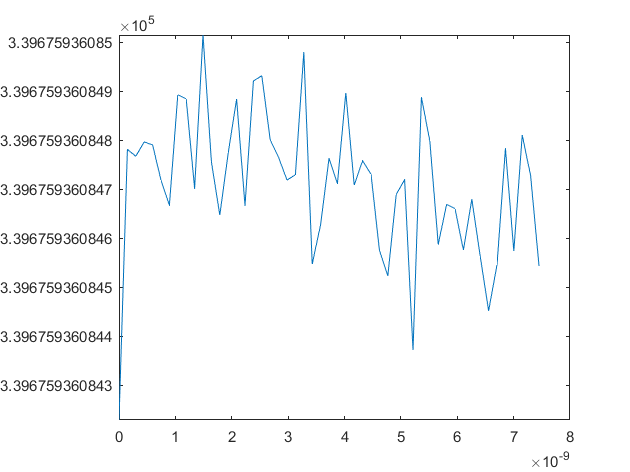
\includegraphics[width=\columnwidth]{fig1}}
\caption{A Figure of function value versus step length during some iteration of the Generalized Bard Function with $n=10^6$. The function suffers from giant fluctuations, and even a step larger than $10^{-9}$ cannot be derived.}
\end{center}
\vskip -0.2in
\end{figure}

The Generalized Cube Function and s303-305 Function do have better numerical properties, which is shown in the good-looking iteration data, while CD is still not a good algorithm solving these problems. Nevertheless, simply by adding a mechanism to restart the algorithm ($c=10$ in the experiments), the performance become much better.

BB method is a strong method with competent function-evaluation time performance, but this is partly because ELS is conducted in other experiments and an ILS method (the non-monotone line search method) is attempted here. Seeing a method only taking gradient as descending direction can converge so fast in Generalized Cube Function is still comforting, though.

Between all CG methods, no single method out-perform others in all three problems. All of them except CD have robust and good performances over large scale problems.

% include your own bib file like this:
%\bibliographystyle{acl}
%\bibliography{acl2018}

\end{document}
